\chapter{Оформление различных элементов}\label{ch:ch1}

%%----[ Взвешенные преобразователи конечных состояний ]-----------------------------------------------

\section{Взвешенные преобразователи конечных состояний}\label{sec:ch1/wfst}

Основопологающую роль в изложенных ниже алгоритмах играет понятие взвешенного преобразователя конечных состояний (Weighted Finite-State Transducer, WFST), а также операции, определенные на данной структуре.

\textit{Взвешенный преобразователь конечных состояний} или \textit{взвешенный трансдьюсер} (далее WFST) на полукольце $(\mathbb{K}, \oplus, \otimes, \bar{0}, \bar{1})$ формально определяется как кортеж $T = \langle\Sigma,\Delta,Q,I,F,E,\lambda,\rho\rangle$, где:
\begin{enumerate}
  \item $\Sigma$ --- конечное множество входных символов.
  \item $\Delta$ --- конечное множество выходных символов.
  \item $Q$ --- конечное множество состояний.
  \item $I \subseteq Q$ --- конечное множество начальных состояний.
  \item $F \subseteq Q$ --- конечное множество финальных состояний.
  \item $E \subseteq Q \times (\Sigma \cup \{\epsilon\}) \times (\Delta \cup \{\epsilon\}) \times \mathbb{K} \times Q$ --- конечное мультимножество переходов, где $\epsilon$ --- мета-символ, означающий пустой входной или выходной символ.
  \item $\lambda : I \rightarrow \mathbb{K}$ --- весовая функция начальных состояний.
  \item $\rho : F \rightarrow \mathbb{K}$ --- весовая фукнция финальных состояний.
\end{enumerate}

\textit{Взвешенный трансдьюсер (WFST)} определяет функцию $f : \Sigma^* \rightarrow 2^{\Delta^*} \rightarrow \mathbb{K}$, преобразующую входную последовательность символов в множество взвешенных последовательностей выходных символов. Частными случаями такой структуры являются:

\begin{enumerate}
  \item \textit{Трансдьюсер (FST)} определяет функцию $f : \Sigma^* \rightarrow 2^{\Delta^*}$, преобразующую входную последовательность символов в множество последовательностей выходных символов, не учитывая веса.
  \item \textit{Aкцептор (FSА)} определяет функцию $f : \Sigma^* \rightarrow \{0, 1\}$, которая оценивает входную последовательность символов как подходящую или как не подходящую. Для акцепторов $\Delta=\emptyset$, и есть только лента для входных символов.
  \item \textit{Взвешенный акцептор (WFSА)} определяет функцию $f : \Sigma^* \rightarrow \mathbb{K}$, которая оценивает входную последовательность символов, возвращая соответствующий последовательности вес.
\end{enumerate}

Для трансдьюсеров определен целый ряд операторов, которые которые можно разделить на две группы:

\begin{enumerate}
  \item Унарные операции, $f : T \rightarrow T$. Унарные операции над трансдьсерами также называются операциями оптимизации. Среди ключевых операций можно выделить операции \textit{детерминизации} и \textit{минимизации}.
  \item Бинарные операции, $f : T \times T \rightarrow T$. Бинарные операции позволяют из двух трансдьюсеров получить третий. Ключевой операцией над двумя трансдьсерами является \textit{композиция}.
\end{enumerate}

Для двух трансдьюсеров $T_1$ и $T_2$ операция композиции определяется следующим образом:
\[
  (T_1 \circ T_2)(x,y)=\bigoplus\limits_{z \in \Delta^*} T_1(x,z) \otimes T_2(z,y).
\]

Таким образом, если трансдьюсер $T_1$ преобразует последовательность символов $x$ в последовательность символов $z$ с весом $w_1$, а трансдьюсер $T_2$ преобразует последовательность символов $z$ в последовательность символов $x$ с весом $w_2$, тогда полученный в результате композиции трансдьюсер $T_1 \circ T_2$ будет преобразовывать последовательность символов $x$ в последовательность символов $y$ с весом $w_1 \otimes w_2$.

%%----[ Автоматическое распознавание речи ]-----------------------------------------------

\section{Автоматическое распознавание речи}\label{sec:ch1/asr}

Процесс автоматического распознавания речи представляет собой преобразование речевого сигнала в текст. Один из способов формального определения задачи распознавания речи следует из теории информации. Последовательность слов $W$ генерируется в сознании говорящего и передается через акустический канал, состоящий из источника речи и акустического процессора. Озвученная последовательность $W$ генерируется в виде сигнала $S$ в акустической среде. Акустический процессор выполняет обработку сигнала $S$ для получения акустических и фонетических признаков $O$. Лингвистический декодер получает векторную последовательность признаков $O$ и выводит последовательность слов $\hat{W}$, близкую к исходной последовательности слов $W$. В такой модели акустический процессор и лингвистический декодер являются частью системы автоматического распознавания речи.

Лингвистический декодер ищет наиболее правдаподобную последовательсность слов $\hat{W}$ в множестве возможных последовательностей слов $\mathcal{W}$ для входной последовательности признаков $O$:
\[
  \hat{W} = \argmax\limits_{W \in \mathcal{W}}P(W|O).
\]

$P(W|O)$ может быть выраженно через теорему Байеса:
\[
  P(W|O) = \frac{p(O|W)P(W)}{p(O)}.
\]
Подставляя в общее выражение, получаем:
\[
  \hat{W} = \argmax\limits_{W \in \mathcal{W}}p(O|W)P(W),
\]
где $p(O|W)$ --- акустическая вероятность $O$ для $W$, а $P(W)$ --- априорная вероятность $W$. Вероятность $p(O)$ в выражении опущена, так как она не зависит от $\hat{W}$. Таким образом для поиска $\hat{W}$ мы рассматриваем только $p(O|W)P(W)$, где $p(O|W)$ рассчитывается с помощью акустической модели, а $P(W)$ --- с помощью языковой, которые благодаря теореме Байеса могут рассчитываться независимо. На~рисунке~\cref{fig:asr_decoder} представлена схема работы системы автоматического распознавания речи.

\begin{figure}[ht]
  \centerfloat{
    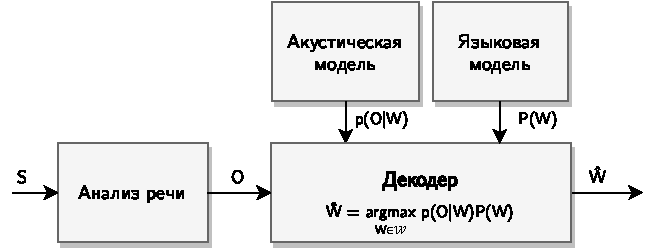
\includegraphics[scale=1.4]{asr_decoder}
  }
  \caption{Общая схема работы системы распознавания речи.}\label{fig:asr_decoder}
\end{figure}

В качестве структуры, объединяющей воедино информацию от акустической и языковой моделей, можно использовать трансдьюсер, преобразующий последовательность признаков $O$, в последовательность слов $W$. В этих терминах акустическая модель может рассматриваться как классификатор для различных предствлений звуков на фонемном уровне $V$. В общем виде \textit{WFST-граф распознавания} может быть предствлен следующей композицей каскада трансдьюсеров:
\[
  N=H \circ L \circ G,
\]
где $H$ --- трансдьюсер, преобразующий связанные состояния в последовательность фонем, $H$ --- трансдьюсер, преобразующий последовательность фонем в слова, а $G$ --- акцептор, взвешивающий слова с учетом веса языковой модели.

Декодер выполняет поиск наиболее вероятных последовательностей слов по WFST-графу распознавания $N$ с ограничением луча поиска с помощью алгоритма Витерби. Сохраненные в процессе поиска переходы в графе с выходными метками слов называются \textit{словными сетями} (lattice). Словная сеть предствляет собой взвешенный акцептор с метками слов. Каждый переход содержит сумму акустического и языкового весов $w = w_{ac} \oplus w_{l}$. Состояния содержат информацию о временных метках. Лучший путь (1-best) в словной сети представляет собой искомую последовательность слов $\hat{W}$.

Важные замечания к гибридным системам автоматического распознавания речи на основе WFST-декодера:

\begin{enumerate}
  \item В силу того, что множество выходных символов трансдьюсера $\Delta$ по определению конечно, граф распознавания оперирует конечным множеством слов $\mathcal{W}$. Таким образом система распознавания может выбирать только среди тех слов, которые знает (in-vocabulary, IV-слова). Слова, которых в словаре нет (out-of-vocabulary, OOV-слова), никогда не будут распознаны корректно. Существует целый ряд подходов к решению проблемы OOV-слов, например, пополнение словаря «на лету».
  \item В общем случае, WFST-декодер на выходе выдает метки, которые для простоты повествования отождествляются со словами. Вместо этого декодер может оперировать фонемами или частями слов. В этом случае требуется пост-обработка результатов для получения слов. Все ниже описанные алгоритмы индексации и поиска могут быть обобщены до использования произвольных термов, однако в рамках данной работы пост-обработка не рассматривается.
  \item Современные системы автоматического распознавания речи, построенные на сквозных архитектурах нейронных сетей, могут быть использованы вместе с WFST-декодером без увеличения пословной ошибки распознавания, с сохранением возможностей по управлению и расширению языковых моделей. Это позволяет использовать предложенные в настоящей работе подходы для подавляющего большинства всех архитектур систем автоматического распознавания речи.
\end{enumerate}

%%----[ Пословная ошибка распознавания ]-----------------------------------------------

\section{Пословная ошибка распознавания}\label{sec:ch1/wer}

В качестве основной метрики оценки качества работы системы автоматического распознавания речи используется \textit{пословная ошибка распознавания} (Word Error Rate, WER), которая рассчитывается по формуле:
\[
  WER\% = 100\% \times \frac{S+D+I}{N} = 100\% \times \frac{S+D+I}{S+D+C},
\]
где $S$ --- количество замен, $D$ --- количество удалений, $I$ --- количество вставок, $C$ --- количество правильных слов, а $N=S+D+C$ --- общее количество слов в исходной последовательности слов $W$. Для рассчета эти величин используется расстояние Левенштейна и соответствующее ему \textit{редакционное предписание} для всех пар $\langle W, \hat{W} \rangle$ тестовой выборки.

Вместе с пословной ошибкой распознавания используется \textit{точность распознавания}, которая рассчитывается следующим образом:
\[
  Acc\% = 100\% - WER\% = 100\% \times \frac{N-S-D-I}{N} = 100\% \times \frac{C-I}{N}.
\]

Нужно отметить, что $N$ --- общее количество слов в исходном тексте, поэтому $WER\%$ может быть больше $100\%$, а $Acc\%$, соответственно, --- меньше $0\%$. Пословная ошибка распознавания учитывает только лучший результат из словной сети. В задачах поиска при использовании всех гипотез из словной сети, необходимо учитывать ошибки первого и второго рода.

%%----[ Сети спутывания ]-----------------------------------------------

\section{Сети спутывания}\label{sec:ch1/confnet}

Словная сеть полученная в результате работы WFST-декодера --- это акцептор со словами на переходах и весами, полученными из акустической и языковой моделей. Словные сети не содержат циклов, имеют одно начальное состояние и одно финальное. При этом количество переходов из каждого состояния может быть произвольным и зависеть от настроек WFST-декодера и ограничений луча поиска. Такая структура позволяет быстро обходить сеть, но в силу нерегулярной структуры плохо поддается индексации.

Вместо словной сети предполагается использовать более компактное ее представление --- \textit{сети спутывания}. Сети спутывания представляют собой такой же акцептор, но с дополнительными свойствами:

\begin{enumerate}
  \item Все пути в сети спутывания от начального состояния к финальному проходят через все состояния. Обход такого графа может быть выполнен за время $O(|E|)$, где $|E|$ --- общее количество переходов.
  \item Набор переходов между парой состояний называется \textit{бином}. Каждый бин имеет временные метки начала и конца, которые размещаются в соответствующих состояниях.
  \item Каждый бин может содержать произвольное количество переходов.
  \item Каждый бин может включать в себя не более чем один $\epsilon$-переход, означающий, что на данном бине слово может быть пропущено. Такие переходы используются в том числе для обозначения паузы.
  \item Для каждого состояния с временной меткой выполняется правило \\ $t_{i} > t_{i-1}$. То есть состояния упорядочены по времени, начиная от начального состояния и следуя до финального. Если отсортировать переходы в каждом из бинов по убыванию веса, то можно получить лучшую гипотезу за время $O(|B|)$, где $|B|$ --- количество бинов в сети спутывания.
  \item Веса на переходах внутри каждого бина в сумме дают единицу и могут интерпретироваться как вероятности.
\end{enumerate}

Пример словной сети, полученной в результате работы WFST-декодера, и соответствующей ей сети спутывания представлен на~рисунке~\cref{fig:confnet}.

\begin{figure}[ht]
  \centerfloat{
    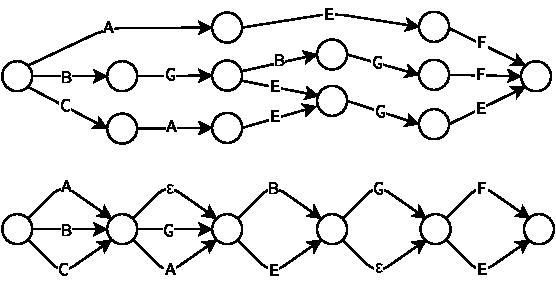
\includegraphics[scale=1.4]{confnet}
  }
  \caption{Пример словной сети декодера и получившейся на ее основе сети спутывания.}\label{fig:confnet}
\end{figure}

Базовыей алгоритм построения сетей спутывания на основе словных сетей может быть разбит на три шага:
\begin{enumerate}
  \item Кластеризация состояний словной сети, выделение бинов сети спутывания.
  \item Кластеризация переходов словной сети. Если $с(v)$ --- номер кластера вершины $v$, то переход $u \rightarrow v$ из исходной словной сети помещается в один из слотов между кластерами $c(u) \ldots c(v)$.
  \item Вычисление вероятностей слов внутри бинов.
\end{enumerate}

\textbf{Кластеризация состояний}. Оригинальный алгоритм предполагает следующий подход. Состояния сортируются по временным меткам, после чего происходит проход по состояниям в порядке возрастания временных меток. Если нет переходов из состояний последнего кластера в рассматриваемое состояние, тогда состояние добавляется в предыдущий кластер. Если же такой переход есть, то создается новый кластер.

Однако, такой подход может кластеризовать состояния, которые очень сильно отличаются по временным меткам. Это можно исправить, используя агломеративную кластеризацию и выбирая на каждом шаге такое объединение, которое создаст более компактный с точки зрения времени кластер. В качестве целевой функции использовалась минимизация длительности кластера $r(c)-l(c)$, где $t(v)$ --- временная метка состояния $v$, а $l(c)$ и $r(c)$ --- минимальные и максимальные значения $t(v)$ состояний $v$ входящих в кластер $с$ соответсвенно.

\textbf{Кластеризация переходов}. Этот этап условно разбивается на три шага:

\begin{enumerate}
 \item Сначала определяются переходы, которые могут быть отнесены в единственный слот, то есть такие $u \rightarrow v$, что $ c(v)=c(u)+1$. Кластеры состояний строятся таким образом, что для каждой пары соседних кластеров обязательно найдется такой переход.
 \item Если переход содержит слово, которое уже попало в какой-то слот, и при этом временные границы этого слота пересекаются с временным отрезком перехода, то переход помещается в этот слот, если таких слотов несколько, то выбирается слот с максимальным пересечением по временным интервалам.
 \item Оставшиеся переходы помещаются в слоты по степени перекрытия временных интервалов.
\end{enumerate}

\textbf{Вычисления вероятностей слов}. На данном шаге выполняется вычисление вероятностей каждого перехода и объединение этих вероятностей по словам. Как уже было сказанно, веса в словной сети не могут быть трактованы как вероятности, являясь логарифмами правдоподобия обусловленными состоянием, из которого они выходят. В качестве приближения вероятности перехода используется сумма правдоподобий всех путей в словной сети, которые содержат этот переход, нормированная на сумму правдоподобий всех путей в латтисе. Получив вероятности переходов, мы легко получаем вероятности слова в кластере сложением всех вероятностей переходов, содержащих это слово.

%%----[ ... ]-----------------------------------------------

\begin{comment}

\section{Форматирование текста}\label{sec:ch1/sec1}

Мы можем сделать \textbf{жирный текст} и \textit{курсив}.

\section{Ссылки}\label{sec:ch1/sec2}

Сошлёмся на библиографию.
Новые ссылки для проверки: \cite{InvertedFiles,MohriWfstAsr,WfstDecAnatomy,ConfNetConsensus,ManguConfNetIndex,Pan2007analytical}.
Одна ссылка: \cite[с.~54]{Sokolov}\cite[с.~36]{Gaidaenko}.
Две ссылки: \cite{Sokolov,Gaidaenko}.
Ссылка на собственные работы: \cite{scopus_rvect, scopus_voices, scopus_arch}.
Много ссылок: %\cite[с.~54]{Lermontov,Management,Borozda} % такой «фокус»
%вызывает biblatex warning относительно опции sortcites, потому что неясно, к
%какому источнику относится уточнение о страницах, а bibtex об этой проблеме
%даже не предупреждает
\cite{Lermontov, Management, Borozda, Marketing, Constitution, FamilyCode,
    Gost.7.0.53, Razumovski, Lagkueva, Pokrovski, Methodology, Berestova,
    Kriger}%
\ifnumequal{\value{bibliosel}}{0}{% Примеры для bibtex8
    \cite{Sirotko, Lukina, Encyclopedia, Nasirova}%
}{% Примеры для biblatex через движок biber
    \cite{Sirotko2, Lukina2, Encyclopedia2, Nasirova2}%
}%
.
И~ещё немного ссылок:~\cite{Article,Book,Booklet,Conference,Inbook,Incollection,Manual,Mastersthesis,
    Misc,Phdthesis,Proceedings,Techreport,Unpublished}
% Следует обратить внимание, что пробел после запятой внутри \cite{}
% обрабатывается ожидаемо, а пробел перед запятой, может вызывать проблемы при
% обработке ссылок.
\cite{medvedev2006jelektronnye, CEAT:CEAT581, doi:10.1080/01932691.2010.513279,
    Gosele1999161,Li2007StressAnalysis, Shoji199895, test:eisner-sample,
    test:eisner-sample-shorted, AB_patent_Pomerantz_1968, iofis_patent1960}%
\ifnumequal{\value{bibliosel}}{0}{% Примеры для bibtex8
}{% Примеры для biblatex через движок biber
    \cite{patent2h, patent3h, patent2}%
}%
.

\ifnumequal{\value{bibliosel}}{0}{% Примеры для bibtex8
Попытка реализовать несколько ссылок на конкретные страницы
для \texttt{bibtex} реализации библиографии:
[\citenum{Sokolov}, с.~54; \citenum{Gaidaenko}, с.~36].
}{% Примеры для biblatex через движок biber
Несколько источников (мультицитата):
% Тут специально написано по-разному тире, для демонстрации, что
% применение специальных тире в настоящий момент в biblatex приводит к непоказу
% "с.".
\cites[vii--x, 5, 7]{Sokolov}[v"--~x, 25, 526]{Gaidaenko}[vii--x, 5, 7]{Techreport},
работает только в \texttt{biblatex} реализации библиографии.
}%

Ссылки на собственные работы:~\cite{scopus_rvect}.

Сошлёмся на приложения: Приложение~\cref{app:A}, Приложение~\cref{app:B2}.

Сошлёмся на формулу: формула~\cref{eq:equation1}.

Сошлёмся на изображение: рисунок~\cref{fig:knuth}.

Стандартной практикой является добавление к ссылкам префикса, характеризующего тип элемента.
Это не является строгим требованием, но~позволяет лучше ориентироваться в документах большого размера.
Например, для ссылок на~рисунки используется префикс \textit{fig},
для ссылки на~таблицу "--- \textit{tab}.

В таблице \cref{tab:tab_pref} приложения~\cref{app:B4} приведён список рекомендуемых
к использованию стандартных префиксов.

В некоторых ситуациях возникает необходимость отойти от требований ГОСТ по оформлению ссылок на
литературу.
В таком случае можно воспользоваться дополнительными опциями пакета \verb+biblatex+.

Например, в ссылке на книгу~\cite{sobenin_kdv} использование опции \verb+maxnames=4+ позволяет
вывести имена всех четырёх авторов.
По ГОСТ имена последних трёх авторов опускаются.

Кроме того, часто возникают проблемы с транслитерованными инициалами. Некоторые буквы русского
алфавита по правилам транслитерации записываются двумя буквами латинского алфавита (ю-yu, ё-yo и
т.д.).
Такие инициалы \verb+biblatex+ будет сокращать до одной буквы, что неверно.
Поправить его работу можно использовав опцию \verb+giveninits=false+.
Пример использования этой опции можно видеть в ссылке~\cite{initials}.

\section{Формулы}\label{sec:ch1/sec3}

Благодаря пакету \textit{icomma}, \LaTeX~одинаково хорошо воспринимает
в~качестве десятичного разделителя и запятую (\(3,1415\)), и точку (\(3.1415\)).

\subsection{Ненумерованные одиночные формулы}\label{subsec:ch1/sec3/sub1}

Вот так может выглядеть формула, которую необходимо вставить в~строку
по~тексту: \(x \approx \sin x\) при \(x \to 0\).

А вот так выглядит ненумерованная отдельностоящая формула c подстрочными
и надстрочными индексами:
\[
    (x_1+x_2)^2 = x_1^2 + 2 x_1 x_2 + x_2^2
\]

Формула с неопределенным интегралом:
\[
    \int f(\alpha+x)=\sum\beta
\]

При использовании дробей формулы могут получаться очень высокие:
\[
    \frac{1}{\sqrt{2}+
        \displaystyle\frac{1}{\sqrt{2}+
            \displaystyle\frac{1}{\sqrt{2}+\cdots}}}
\]

В формулах можно использовать греческие буквы:
%Все \original... команды заранее, ради этого примера, определены в Dissertation\userstyles.tex
\[
    \alpha\beta\gamma\delta\originalepsilon\epsilon\zeta\eta\theta%
    \vartheta\iota\kappa\varkappa\lambda\mu\nu\xi\pi\varpi\rho\varrho%
    \sigma\varsigma\tau\upsilon\originalphi\phi\chi\psi\omega\Gamma\Delta%
    \Theta\Lambda\Xi\Pi\Sigma\Upsilon\Phi\Psi\Omega
\]
\[%https://texfaq.org/FAQ-boldgreek
    \boldsymbol{\alpha\beta\gamma\delta\originalepsilon\epsilon\zeta\eta%
        \theta\vartheta\iota\kappa\varkappa\lambda\mu\nu\xi\pi\varpi\rho%
        \varrho\sigma\varsigma\tau\upsilon\originalphi\phi\chi\psi\omega\Gamma%
        \Delta\Theta\Lambda\Xi\Pi\Sigma\Upsilon\Phi\Psi\Omega}
\]

Для добавления формул можно использовать пары \verb+$+\dots\verb+$+ и \verb+$$+\dots\verb+$$+,
но~они считаются устаревшими.
Лучше использовать их функциональные аналоги \verb+\(+\dots\verb+\)+ и \verb+\[+\dots\verb+\]+.

\subsection{Ненумерованные многострочные формулы}\label{subsec:ch1/sec3/sub2}

Вот так можно написать две формулы, не нумеруя их, чтобы знаки <<равно>> были
строго друг под другом:
\begin{align}
    f_W & =  \min \left( 1, \max \left( 0, \frac{W_{soil} / W_{max}}{W_{crit}} \right)  \right), \nonumber \\
    f_T & =  \min \left( 1, \max \left( 0, \frac{T_s / T_{melt}}{T_{crit}} \right)  \right), \nonumber
\end{align}

Выровнять систему ещё и по переменной \( x \) можно, используя окружение
\verb|alignedat| из пакета \verb|amsmath|. Вот так:
\[
|x| = \left\{
\begin{alignedat}{2}
    &&x, \quad &\text{eсли } x\geqslant 0 \\
    &-&x, \quad & \text{eсли } x<0
\end{alignedat}
\right.
\]
Здесь первый амперсанд (в исходном \LaTeX\ описании формулы) означает
выравнивание по~левому краю, второй "--- по~\( x \), а~третий "--- по~слову
<<если>>. Команда \verb|\quad| делает большой горизонтальный пробел.

Ещё вариант:
\[
    |x|=
    \begin{cases}
        \phantom{-}x, \text{если } x \geqslant 0 \\
        -x, \text{если } x<0
    \end{cases}
\]

Кроме того, для  нумерованных формул \verb|alignedat| делает вертикальное
выравнивание номера формулы по центру формулы. Например, выравнивание
компонент вектора:
\begin{equation}
    \label{eq:2p3}
    \begin{alignedat}{2}
        {\mathbf{N}}_{o1n}^{(j)} = \,{\sin} \phi\,n\!\left(n+1\right)
        {\sin}\theta\,
        \pi_n\!\left({\cos} \theta\right)
        \frac{
        z_n^{(j)}\!\left( \rho \right)
        }{\rho}\,
        &{\boldsymbol{\hat{\mathrm e}}}_{r}\,+   \\
        +\,
        {\sin} \phi\,
        \tau_n\!\left({\cos} \theta\right)
        \frac{
        \left[\rho z_n^{(j)}\!\left( \rho \right)\right]^{\prime}
        }{\rho}\,
        &{\boldsymbol{\hat{\mathrm e}}}_{\theta}\,+   \\
        +\,
        {\cos} \phi\,
        \pi_n\!\left({\cos} \theta\right)
        \frac{
        \left[\rho z_n^{(j)}\!\left( \rho \right)\right]^{\prime}
        }{\rho}\,
        &{\boldsymbol{\hat{\mathrm e}}}_{\phi}\:.
    \end{alignedat}
\end{equation}

Ещё об отступах. Иногда для лучшей <<читаемости>> формул полезно
немного исправить стандартные интервалы \LaTeX\ с учётом логической
структуры самой формулы. Например в формуле~\cref{eq:2p3} добавлен
небольшой отступ \verb+\,+ между основными сомножителями, ниже
результат применения всех вариантов отступа:
\begin{align*}
    \backslash!             & \quad f(x) = x^2\! +3x\! +2         \\
    \mbox{по-умолчанию}     & \quad f(x) = x^2+3x+2               \\
    \backslash,             & \quad f(x) = x^2\, +3x\, +2         \\
    \backslash{:}           & \quad f(x) = x^2\: +3x\: +2         \\
    \backslash;             & \quad f(x) = x^2\; +3x\; +2         \\
    \backslash \mbox{space} & \quad f(x) = x^2\ +3x\ +2           \\
    \backslash \mbox{quad}  & \quad f(x) = x^2\quad +3x\quad +2   \\
    \backslash \mbox{qquad} & \quad f(x) = x^2\qquad +3x\qquad +2
\end{align*}

Можно использовать разные математические алфавиты:
\begin{align}
    \mathcal{ABCDEFGHIJKLMNOPQRSTUVWXYZ} \nonumber  \\
    \mathfrak{ABCDEFGHIJKLMNOPQRSTUVWXYZ} \nonumber \\
    \mathbb{ABCDEFGHIJKLMNOPQRSTUVWXYZ} \nonumber
\end{align}

Посмотрим на систему уравнений на примере аттрактора Лоренца:

\[
\left\{
\begin{array}{rl}
    \dot x = & \sigma (y-x)  \\
    \dot y = & x (r - z) - y \\
    \dot z = & xy - bz
\end{array}
\right.
\]

А для вёрстки матриц удобно использовать многоточия:
\[
    \left(
        \begin{array}{ccc}
            a_{11} & \ldots & a_{1n} \\
            \vdots & \ddots & \vdots \\
            a_{n1} & \ldots & a_{nn} \\
        \end{array}
    \right)
\]

\subsection{Нумерованные формулы}\label{subsec:ch1/sec3/sub3}

А вот так пишется нумерованная формула:
\begin{equation}
    \label{eq:equation1}
    e = \lim_{n \to \infty} \left( 1+\frac{1}{n} \right) ^n
\end{equation}

Нумерованных формул может быть несколько:
\begin{equation}
    \label{eq:equation2}
    \lim_{n \to \infty} \sum_{k=1}^n \frac{1}{k^2} = \frac{\pi^2}{6}
\end{equation}

Впоследствии на формулы~\cref{eq:equation1, eq:equation2} можно ссылаться.

Сделать так, чтобы номер формулы стоял напротив средней строки, можно,
используя окружение \verb|multlined| (пакет \verb|mathtools|) вместо
\verb|multline| внутри окружения \verb|equation|. Вот так:
\begin{equation} % \tag{S} % tag - вписывает свой текст
    \label{eq:equation3}
    \begin{multlined}
        1+ 2+3+4+5+6+7+\dots + \\
        + 50+51+52+53+54+55+56+57 + \dots + \\
        + 96+97+98+99+100=5050
    \end{multlined}
\end{equation}

Уравнения~\cref{eq:subeq_1,eq:subeq_2} демонстрируют возможности
окружения \verb|\subequations|.
\begin{subequations}
    \label{eq:subeq_1}
    \begin{gather}
        y = x^2 + 1 \label{eq:subeq_1-1} \\
        y = 2 x^2 - x + 1 \label{eq:subeq_1-2}
    \end{gather}
\end{subequations}
Ссылки на отдельные уравнения~\cref{eq:subeq_1-1,eq:subeq_1-2,eq:subeq_2-1}.
\begin{subequations}
    \label{eq:subeq_2}
    \begin{align}
        y & = x^3 + x^2 + x + 1 \label{eq:subeq_2-1} \\
        y & = x^2
    \end{align}
\end{subequations}

\subsection{Форматирование чисел и размерностей величин}\label{sec:units}

Числа форматируются при помощи команды \verb|\num|:
\num{5,3};
\num{2,3e8};
\num{12345,67890};
\num{2,6 d4};
\num{1+-2i};
\num{.3e45};
\num[exponent-base=2]{5 e64};
\num[exponent-base=2,exponent-to-prefix]{5 e64};
\num{1.654 x 2.34 x 3.430}
\num{1 2 x 3 / 4}.
Для написания последовательности чисел можно использовать команды \verb|\numlist| и \verb|\numrange|:
\numlist{10;30;50;70}; \numrange{10}{30}.
Значения углов можно форматировать при помощи команды \verb|\ang|:
\ang{2.67};
\ang{30,3};
\ang{-1;;};
\ang{;-2;};
\ang{;;-3};
\ang{300;10;1}.

Обратите внимание, что ГОСТ запрещает использование знака <<->> для обозначения отрицательных чисел
за исключением формул, таблиц и~рисунков.
Вместо него следует использовать слово <<минус>>.

Размерности можно записывать при помощи команд \verb|\si| и \verb|\SI|:
\si{\farad\squared\lumen\candela};
\si{\joule\per\mole\per\kelvin};
\si[per-mode = symbol-or-fraction]{\joule\per\mole\per\kelvin};
\si{\metre\per\second\squared};
\SI{0.10(5)}{\neper};
\SI{1.2-3i e5}{\joule\per\mole\per\kelvin};
\SIlist{1;2;3;4}{\tesla};
\SIrange{50}{100}{\volt}.
Список единиц измерений приведён в таблицах~\cref{tab:unit:base,
    tab:unit:derived,tab:unit:accepted,tab:unit:physical,tab:unit:other}.
Приставки единиц приведены в~таблице~\cref{tab:unit:prefix}.

С дополнительными опциями форматирования можно ознакомиться в~описании пакета \texttt{siunitx};
изменить или добавить единицы измерений можно в~файле \texttt{siunitx.cfg}.

\begin{table}
    \centering
    \captionsetup{justification=centering} % выравнивание подписи по-центру
    \caption{Основные величины СИ}\label{tab:unit:base}
    \begin{tabular}{llc}
        \toprule
        Название  & Команда                 & Символ         \\
        \midrule
        Ампер     & \verb|\ampere| & \si{\ampere}   \\
        Кандела   & \verb|\candela| & \si{\candela}  \\
        Кельвин   & \verb|\kelvin| & \si{\kelvin}   \\
        Килограмм & \verb|\kilogram| & \si{\kilogram} \\
        Метр      & \verb|\metre| & \si{\metre}    \\
        Моль      & \verb|\mole| & \si{\mole}     \\
        Секунда   & \verb|\second| & \si{\second}   \\
        \bottomrule
    \end{tabular}
\end{table}

\begin{table}
    \small
    \centering
    \begin{threeparttable}% выравнивание подписи по границам таблицы
        \caption{Производные единицы СИ}\label{tab:unit:derived}
        \begin{tabular}{llc|llc}
            \toprule
            Название       & Команда                 & Символ              & Название & Команда & Символ \\
            \midrule
            Беккерель      & \verb|\becquerel| & \si{\becquerel}     &
            Ньютон         & \verb|\newton| & \si{\newton}                                      \\
            Градус Цельсия & \verb|\degreeCelsius| & \si{\degreeCelsius} &
            Ом             & \verb|\ohm| & \si{\ohm}                                         \\
            Кулон          & \verb|\coulomb| & \si{\coulomb}       &
            Паскаль        & \verb|\pascal| & \si{\pascal}                                      \\
            Фарад          & \verb|\farad| & \si{\farad}         &
            Радиан         & \verb|\radian| & \si{\radian}                                      \\
            Грей           & \verb|\gray| & \si{\gray}          &
            Сименс         & \verb|\siemens| & \si{\siemens}                                     \\
            Герц           & \verb|\hertz| & \si{\hertz}         &
            Зиверт         & \verb|\sievert| & \si{\sievert}                                     \\
            Генри          & \verb|\henry| & \si{\henry}         &
            Стерадиан      & \verb|\steradian| & \si{\steradian}                                   \\
            Джоуль         & \verb|\joule| & \si{\joule}         &
            Тесла          & \verb|\tesla| & \si{\tesla}                                       \\
            Катал          & \verb|\katal| & \si{\katal}         &
            Вольт          & \verb|\volt| & \si{\volt}                                        \\
            Люмен          & \verb|\lumen| & \si{\lumen}         &
            Ватт           & \verb|\watt| & \si{\watt}                                        \\
            Люкс           & \verb|\lux| & \si{\lux}           &
            Вебер          & \verb|\weber| & \si{\weber}                                       \\
            \bottomrule
        \end{tabular}
    \end{threeparttable}
\end{table}

\begin{table}
    \centering
    \begin{threeparttable}% выравнивание подписи по границам таблицы
        \caption{Внесистемные единицы}\label{tab:unit:accepted}

        \begin{tabular}{llc}
            \toprule
            Название        & Команда                 & Символ          \\
            \midrule
            День            & \verb|\day| & \si{\day}       \\
            Градус          & \verb|\degree| & \si{\degree}    \\
            Гектар          & \verb|\hectare| & \si{\hectare}   \\
            Час             & \verb|\hour| & \si{\hour}      \\
            Литр            & \verb|\litre| & \si{\litre}     \\
            Угловая минута  & \verb|\arcminute| & \si{\arcminute} \\
            Угловая секунда & \verb|\arcsecond| & \si{\arcsecond} \\ %
            Минута          & \verb|\minute| & \si{\minute}    \\
            Тонна           & \verb|\tonne| & \si{\tonne}     \\
            \bottomrule
        \end{tabular}
    \end{threeparttable}
\end{table}

\begin{table}
    \centering
    \captionsetup{justification=centering}
    \caption{Внесистемные единицы, получаемые из эксперимента}\label{tab:unit:physical}
    \begin{tabular}{llc}
        \toprule
        Название                & Команда                 & Символ                 \\
        \midrule
        Астрономическая единица & \verb|\astronomicalunit| & \si{\astronomicalunit} \\
        Атомная единица массы   & \verb|\atomicmassunit| & \si{\atomicmassunit}   \\
        Боровский радиус        & \verb|\bohr| & \si{\bohr}             \\
        Скорость света          & \verb|\clight| & \si{\clight}           \\
        Дальтон                 & \verb|\dalton| & \si{\dalton}           \\
        Масса электрона         & \verb|\electronmass| & \si{\electronmass}     \\
        Электрон Вольт          & \verb|\electronvolt| & \si{\electronvolt}     \\
        Элементарный заряд      & \verb|\elementarycharge| & \si{\elementarycharge} \\
        Энергия Хартри          & \verb|\hartree| & \si{\hartree}          \\
        Постоянная Планка       & \verb|\planckbar| & \si{\planckbar}        \\
        \bottomrule
    \end{tabular}
\end{table}

\begin{table}
    \centering
    \begin{threeparttable}% выравнивание подписи по границам таблицы
        \caption{Другие внесистемные единицы}\label{tab:unit:other}
        \begin{tabular}{llc}
            \toprule
            Название                  & Команда                 & Символ             \\
            \midrule
            Ангстрем                  & \verb|\angstrom| & \si{\angstrom}     \\
            Бар                       & \verb|\bar| & \si{\bar}          \\
            Барн                      & \verb|\barn| & \si{\barn}         \\
            Бел                       & \verb|\bel| & \si{\bel}          \\
            Децибел                   & \verb|\decibel| & \si{\decibel}      \\
            Узел                      & \verb|\knot| & \si{\knot}         \\
            Миллиметр ртутного столба & \verb|\mmHg| & \si{\mmHg}         \\
            Морская миля              & \verb|\nauticalmile| & \si{\nauticalmile} \\
            Непер                     & \verb|\neper| & \si{\neper}        \\
            \bottomrule
        \end{tabular}
    \end{threeparttable}
\end{table}

\begin{table}
    \small
    \centering
    \begin{threeparttable}% выравнивание подписи по границам таблицы
        \caption{Приставки СИ}\label{tab:unit:prefix}
        \begin{tabular}{llcc|llcc}
            \toprule
            Приставка & Команда                  & Символ      & Степень &
            Приставка & Команда                  & Символ      & Степень   \\
            \midrule
            Иокто     & \verb|\yocto|  & \si{\yocto} & -24     &
            Дека      & \verb|\deca|  & \si{\deca}  & 1         \\
            Зепто     & \verb|\zepto|  & \si{\zepto} & -21     &
            Гекто     & \verb|\hecto|  & \si{\hecto} & 2         \\
            Атто      & \verb|\atto|  & \si{\atto}  & -18     &
            Кило      & \verb|\kilo|  & \si{\kilo}  & 3         \\
            Фемто     & \verb|\femto|  & \si{\femto} & -15     &
            Мега      & \verb|\mega|  & \si{\mega}  & 6         \\
            Пико      & \verb|\pico|  & \si{\pico}  & -12     &
            Гига      & \verb|\giga|  & \si{\giga}  & 9         \\
            Нано      & \verb|\nano|  & \si{\nano}  & -9      &
            Терра     & \verb|\tera|  & \si{\tera}  & 12        \\
            Микро     & \verb|\micro|  & \si{\micro} & -6      &
            Пета      & \verb|\peta|  & \si{\peta}  & 15        \\
            Милли     & \verb|\milli|  & \si{\milli} & -3      &
            Екса      & \verb|\exa|  & \si{\exa}   & 18        \\
            Санти     & \verb|\centi|  & \si{\centi} & -2      &
            Зетта     & \verb|\zetta|  & \si{\zetta} & 21        \\
            Деци      & \verb|\deci| & \si{\deci}  & -1      &
            Иотта     & \verb|\yotta| & \si{\yotta} & 24        \\
            \bottomrule
        \end{tabular}
    \end{threeparttable}
\end{table}

\subsection{Заголовки с формулами: \texorpdfstring{\(a^2 + b^2 = c^2\)}{%
        a\texttwosuperior\ + b\texttwosuperior\ = c\texttwosuperior},
    \texorpdfstring{\(\left\vert\textrm{{Im}}\Sigma\left(
            \protect\varepsilon\right)\right\vert\approx const\)}{|ImΣ (ε)| ≈ const},
    \texorpdfstring{\(\sigma_{xx}^{(1)}\)}{σ\_\{xx\}\textasciicircum\{(1)\}}
}\label{subsec:with_math}

Пакет \texttt{hyperref} берёт текст для закладок в pdf-файле из~аргументов
команд типа \verb|\section|, которые могут содержать математические формулы,
а~также изменения цвета текста или шрифта, которые не отображаются в~закладках.
Чтобы использование формул в заголовках не вызывало в~логе компиляции появление
предупреждений типа <<\texttt{Token not allowed in~a~PDF string
    (Unicode):(hyperref) removing...}>>, следует использовать конструкцию
\verb|\texorpdfstring{}{}|, где в~первых фигурных скобках указывается
формула, а~во~вторых "--- запись формулы для закладок.

\section{Рецензирование текста}\label{sec:markup}

В шаблоне для диссертации и автореферата заданы команды рецензирования.
Они видны при компиляции шаблона в режиме черновика или при установке
соответствующей настройки (\verb+showmarkup+) в~файле \verb+common/setup.tex+.

Команда \verb+\todo+ отмечает текст красным цветом.
\todo{Например, так.}

Команда \verb+\note+ позволяет выбрать цвет текста.
\note{Чёрный, } \note[red]{красный, } \note[green]{зелёный, }
\note[blue]{синий.} \note[orange]{Обратите внимание на ширину и расстановку
    формирующихся пробелов, в~результате приведённой записи (зависит также
    от~применяемого компилятора).}

Окружение \verb+commentbox+ также позволяет выбрать цвет.

\begin{commentbox}[red]
    Красный текст.

    Несколько параграфов красного текста.
\end{commentbox}

\begin{commentbox}[blue]
    Синяя формула.

    \begin{equation}
        \alpha + \beta = \gamma
    \end{equation}
\end{commentbox}

\verb+commentbox+ позволяет закомментировать участок кода в~режиме чистовика.
Чтобы убрать кусок кода для всех режимов, можно использовать окружение
\verb+comment+.

\section{Работа со списком сокращений и~условных обозначений}\label{sec:acronyms}

С помощью пакета \texttt{nomencl} можно создавать удобный сортированный список
сокращений и условных обозначений во время написания текста. Вызов
\verb+\nomenclature+ добавляет нужный символ или сокращение с~описанием
в~список, который затем печатается вызовом \verb+\printnomenclature+
в~соответствующем разделе.
Для того, чтобы эти операции прошли, потребуется дополнительный вызов
\verb+makeindex -s nomencl.ist -o %.nls %.nlo+ в~командной строке, где вместо
\verb+%+ следует подставить имя главного файла проекта (\verb+dissertation+
для этого шаблона).
Затем потребуется один или два дополнительных вызова компилятора проекта.
\begin{equation}
    \omega = c k,
\end{equation}
где \( \omega \) "--- частота света, \( c \) "--- скорость света, \( k \) "---
модуль волнового вектора.
\nomenclature{\(\omega\)}{частота света\nomrefeq}
\nomenclature{\(c\)}{скорость света\nomrefpage}
\nomenclature{\(k\)}{модуль волнового вектора\nomrefeqpage}
Использование
\begin{verbatim}
\nomenclature{\(\omega\)}{частота света\nomrefeq}
\nomenclature{\(c\)}{скорость света\nomrefpage}
\nomenclature{\(k\)}{модуль волнового вектора\nomrefeqpage}
\end{verbatim}
после уравнения добавит в список условных обозначений три записи.
Ссылки \verb+\nomrefeq+ на последнее уравнение, \verb+\nomrefpage+ "--- на
страницу, \verb+\nomrefeqpage+ "--- сразу на~последнее уравнение и~на~страницу,
можно опускать и~не~использовать.

Группировкой и сортировкой пунктов в списке можно управлять с~помощью указания
дополнительных аргументов к команде \verb+nomenclature+.
Например, при вызове
\begin{verbatim}
\nomenclature[03]{\( \hbar \)}{постоянная Планка}
\nomenclature[01]{\( G \)}{гравитационная постоянная}
\end{verbatim}
\( G \) будет стоять в списке выше, чем \( \hbar \).
Для корректных вертикальных отступов между строками в описании лучше
не~использовать многострочные формулы в~списке обозначений.

\nomenclature{%
    \( \begin{rcases}
        a_n \\
        b_n
    \end{rcases} \)%
}{коэффициенты разложения Ми в дальнем поле соответствующие электрическим и
    магнитным мультиполям}
\nomenclature[a\( e \)]{\( {\boldsymbol{\hat{\mathrm e}}} \)}{единичный вектор}
\nomenclature{\( E_0 \)}{амплитуда падающего поля}
\nomenclature{\( j \)}{тип функции Бесселя}
\nomenclature{\( k \)}{волновой вектор падающей волны}
\nomenclature{%
    \( \begin{rcases}
        a_n \\
        b_n
    \end{rcases} \)%
}{и снова коэффициенты разложения Ми в дальнем поле соответствующие
    электрическим и магнитным мультиполям. Добавлено много текста, так что
    описание группы условных обозначений значительно превысило высоту этой
    группы...}
\nomenclature{\( L \)}{общее число слоёв}
\nomenclature{\( l \)}{номер слоя внутри стратифицированной сферы}
\nomenclature{\( \lambda \)}{длина волны электромагнитного излучения в вакууме}
\nomenclature{\( n \)}{порядок мультиполя}
\nomenclature{%
    \( \begin{rcases}
        {\mathbf{N}}_{e1n}^{(j)} & {\mathbf{N}}_{o1n}^{(j)} \\
        {\mathbf{M}_{o1n}^{(j)}} & {\mathbf{M}_{e1n}^{(j)}}
    \end{rcases} \)%
}{сферические векторные гармоники}
\nomenclature{\( \mu \)}{магнитная проницаемость в вакууме}
\nomenclature{\( r, \theta, \phi \)}{полярные координаты}
\nomenclature{\( \omega \)}{частота падающей волны}

С помощью \verb+nomenclature+ можно включать в~список сокращения,
не~используя их~в~тексте.
% запись сокращения в список происходит командой \nomenclature,
% а не употреблением самого сокращения
\nomenclature{FEM}{finite element method, метод конечных элементов}
\nomenclature{FIT}{finite integration technique, метод конечных интегралов}
\nomenclature{FMM}{fast multipole method, быстрый метод многополюсника}
\nomenclature{FVTD}{finite volume time-domain, метод конечных объёмов
    во~временной области}
\nomenclature{MLFMA}{multilevel fast multipole algorithm, многоуровневый
    быстрый алгоритм многополюсника}
\nomenclature{BEM}{boundary element method, метод граничных элементов}
\nomenclature{CST MWS}{Computer Simulation Technology Microwave Studio
    программа для компьютерного моделирования уравнен Максвелла}
\nomenclature{DDA}{discrete dipole approximation, приближение дискретиных
    диполей}
\nomenclature{FDFD}{finite difference frequency domain, метод конечных
    разностей в~частотной области}
\nomenclature{FDTD}{finite difference time domain, метод конечных разностей
    во~временной области}
\nomenclature{MoM}{method of moments, метод моментов}
\nomenclature{MSTM}{multiple sphere T-Matrix, метод Т-матриц для множества
    сфер}
\nomenclature{PSTD}{pseudospectral time domain method, псевдоспектральный метод
    во~временной области}
\nomenclature{TLM}{transmission line matrix method, метод матриц линий передач}

\end{comment}

\FloatBarrier
